\chapter{Evaluation}\label{sec:eval}

%TODO Speedup Berechnung, Tabellen statt grafiken

Im folgenden wird der Gebrauch von Rust im Zusammenhang mit dem invasiven Computing evaluiert. Hierbei
wird vor allem mit den bereits unterstützten Sprachen C und X10 verglichen.

\section{Laufzeitverhalten, Kompilierungsdauer und Dateigröße}

Zu Beginn werden das Laufzeitverhalten, die Kompilierungsdauer und die Dateigröße kompilierter Programme zwischen
den drei Programmiersprachen verglichen.

Es wurde ein Python-Script geschrieben, welches es ermöglicht, die unterschiedlichen Benchmark-Programme mit unterschiedlichen
...

Alle Programme wurden auf der folgenden Hardware/Software Konfiguration ausgeführt:

\begin{itemize}
	\item{CPU: Intel Core i5-5200U @ 2.2GHZ x 2}
	\item{RAM: 8GB}
	\item{OS: Antergos Linux, Kernel 4.12.13-1-ARCH}
	\item{gcc: 6.3.0}
	\item{IRTSS: 2017-06-07-nightly}
	\item{rustc: 1.19.0-nightly}
	\item{jdk: openjdk 1.8.0\char`_131}
\end{itemize}

\subsection{Vergleich der Anlaufzeit}

Es wird überprüft, wie lange ein Programm, welches in einer der respektiven Programmiersprachen geschrieben wurde,
benötigt, um zu starten und anschließend sofort wieder aufzuhören.

\begin{center}
	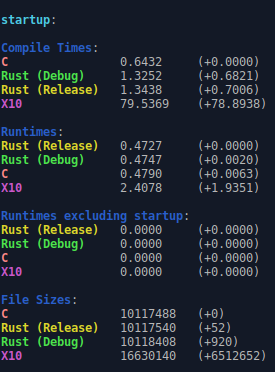
\includegraphics[height=200px]{eval-screenshots/startup.png}  
\end{center}

Anhand dieser Werte kann man prinzipiell erkennen, dass die Anlaufzeiten von C und Rust sich sehr nahe sind, während X10
hierfür ca. 2 Sekunden länger benötigt. Außerdem benötigt das X10 Programm weitaus länger um die Kompilierung auszuführen und
weist eine deutlich größere Dateigröße auf.

\subsection{Berechnen von Primzahlen}

Um die Rechenleistung der verschiedenen Programmiersprachen bei einem intensiveren Problem zu vergleichen, wurden
Programme geschrieben welche Primzahlen berechnen. Hierbei wurden zwei unterschiedliche Ansätze verwendet: Zum einen
eine naive Berechnung, welche jede Zahl individuell auf Teilbarkeit mit kleineren Zahlen prüft und andererseits
das Sieb von Eratosthenes, eine effiziente Methode zum Berechnen von Primzahlen.

\begin{center}
	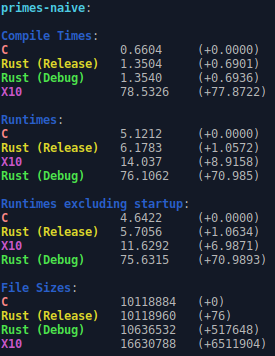
\includegraphics[height=200px]{eval-screenshots/primes-naive.png}
	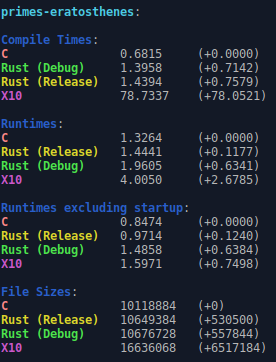
\includegraphics[height=200px]{eval-screenshots/primes-eratosthenes.png}
\end{center}

Hier erkennt man bereits einige Leistungsunterschiede zwischen den Programmiersprachen. Während C die unangefochten
beste Laufzeit aufweist, hinkt Rust nicht signifikant hinterher, während die Lauzeit des X10-Programms auch nach Abzug
der größeren Anlaufzeit schlechter als die beiden Systemsprachen abschneidet.


\subsection{Müll-Ersteller}

X10 verwaltet den Speicher mithilfe eines Garbage Collectors, wobei C und Rust ohne einen solchen auskommen.
Während Garbage Collector ein sehr hilfreiches Werkzeug sind, um den Programmieraufwand zu verringern, so kommt dies
allerdings auch auf Kosten der Laufzeiteffizienz, vor allem die Garbage-Collector-Pause ist hier ein nicht zu unterschätzender
Faktor.

Um diese Leistungsdifferenz zu veranschaulichen, wurde ein Benchmark-Programm geschrieben, welche kontinuierlich
Objekte auf dem Heap erstellt, welche anschließend wieder aus dem gültigen Anwendungsbereich verschwindet.

\begin{center}
	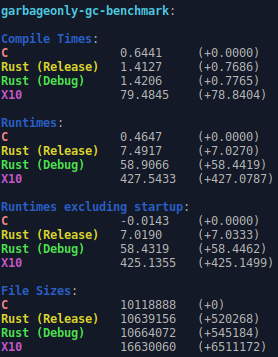
\includegraphics[height=300px]{eval-screenshots/garbageonly.png}
\end{center}

Wie man an den Ergebnissen des Benchmarks erkennen kann, benötigt X10 deutlich länger um die selbe Anzahl und gleich große
Objekte zu erstellen als C oder Rust. Dies weist darauf hin dass der Garbage Collector unter Umständen einen signifikanten
Einfluss auf das Laufzeitverhalten haben kann. C und Rust haben hier also einen Vorteil, vor allem Rust, denn
diese Sprache bietet eine ähnliche Speichersicherheit wie es Sprachen mit Garbage Collector bieten.


\section{Sicherheit}

Im folgenden wird die Sicherheit bezüglich undefiniertem Verhalten als Folge von fehlerhaften Speicherzugriffen analysiert.
Hierbei ist vor allem der Vergleich zwischen Rust und C interessant, da einige von Rusts primären Eigenschaften die
Risiken der C-Programmierung beseitigen sollen.

\subsection{Division durch 0}

Dividiert man in C einen Wert durch die Zahl 0, kann es zu undefiniertem Verhalten führen, welches generell
unerwünschtes Verhalten darstellt. Versucht man dies in Rust, so stürzt das Programm sofort ab, es kann nicht zu undefiniertem
Verhalten kommen.

\subsection{Pufferüberlauf}

Ein weiterer Fall, der in C zu undefiniertem Verhalten führt, sind Pufferüberläufe. Diese geschehen, wenn man beispielsweise
in einem Array der Größe n versucht, auf das n+1te Element zuzugreifen. Wie bereits im letzten Vergleich kann dies in 
Rust nicht geschehen, da das Programm abstürzt.

\subsection{Nicht Initialisierte Variablen}

In C ist es möglich, uninitialiserte Variablen zu verwenden, dies führt allerdings zu undefiniertem Verhalten. In Rust hingegen
wird dies bereits vom Compiler verhindert, da er den Gebrauch von uninitialisierten Variablen verbietet. Ein Rust-Programm
welches also uninitialisierte Variablen verwendet kompiliert also gar nicht und kann so natürlich auch nicht
zu undefiniertem Verhalten führen.


\section{Abstraktionen}

Es werden nun die implementierten Abstraktionen der octolib Bibliothek mit den Implementierungen in C und X10 verglichen.

\subsection{Minimales Infect}

\subsection{Cleanup}

\subsection{Closures}

Closures bieten eine praktische Art und Weise, anonyme Funktionen zu nutzen


